% Standalone VLDB-style preview: E2 cost surfaces only (figures + captions).
\documentclass[sigconf,nonacm]{acmart}
\usepackage{../../../tex/vendor/pvldb}
\settopmatter{printfolios=false,printccs=false,printacmref=false}
\acmConference[Preview]{E2 round 2}{2026}{}
\usepackage{graphicx}
\usepackage{subcaption}
\usepackage{xcolor}
\graphicspath{{../out/}{../out/panels/}}

\begin{document}
\title{E2 Layout Preview (figures only)}
\author{Round-2 agent}
\renewcommand{\shortauthors}{Preview}
\maketitle

\noindent\textcolor{gray}{\textit{Synthetic layout data only --- not experimental results. Cost prediction vs.\ measurement; Spearman quality panel omitted.}}

% Container pattern: adapted from unpacked-paper/exp.tex fig:exp5-m (2 rows, tight hspace).
% Original paper has no confirmed 3D k-sweep float; fig:exp2-k is six 2D LIMIT-$K$ curves.
\begin{figure*}[t]
  \centering
  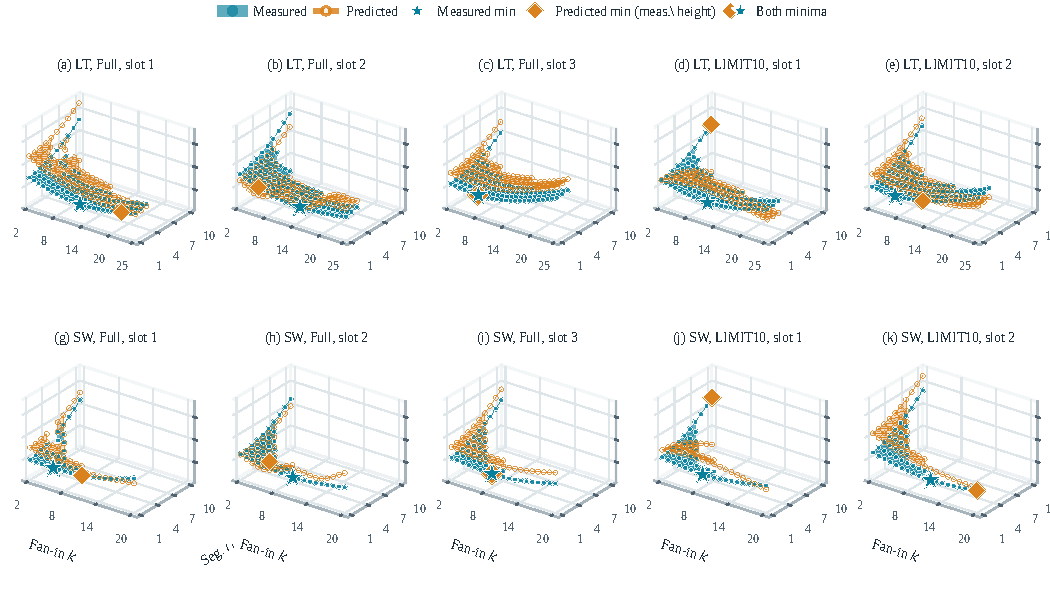
\includegraphics[width=\textwidth]{e2-layout-2x5.pdf}
  \caption{Ten-panel compact candidate (2$\times$5). Blue measured surface with filled vertex markers; orange predicted surface with open vertex markers. Shared triangulation rules and orthographic camera on every panel. Heights are synthetic schematic fields for layout review only.}
  \label{fig:e2-surface-2x5}
\end{figure*}
\begin{figure*}[t]
  \centering
  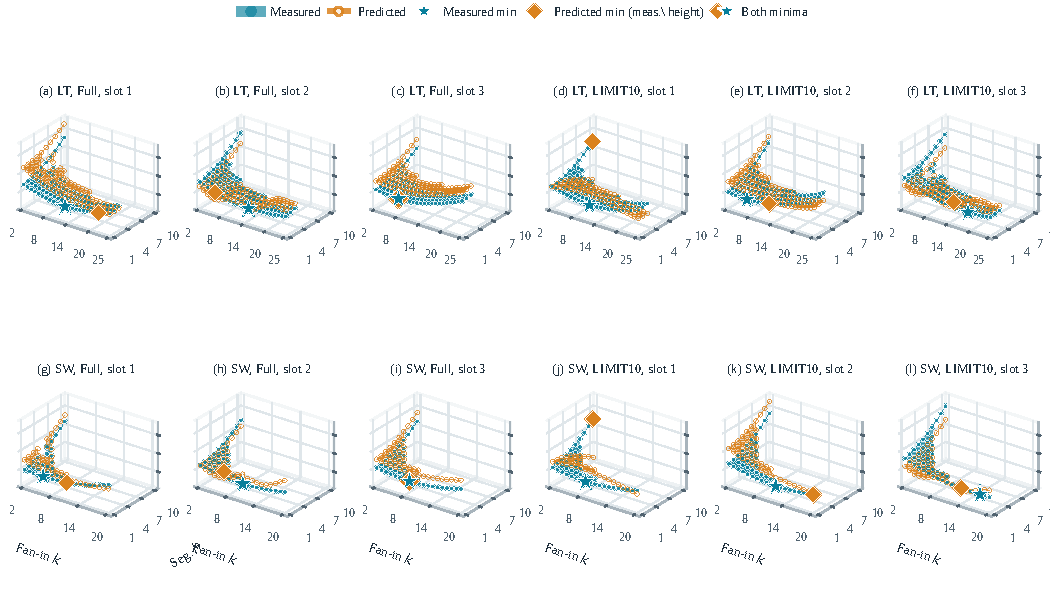
\includegraphics[width=\textwidth]{e2-layout-2x6.pdf}
  \caption{Twelve-panel compact candidate (2$\times$6), row/column spacing aligned to \texttt{fig:exp5-m} in the source \texttt{exp.tex}. Same cost-only 3D style as the 10-panel figure; additional LT/SW LIMIT and Full slots. Synthetic schematic heights; not experimental results.}
  \label{fig:e2-surface-2x6}
\end{figure*}

\begin{figure}[t]
  \centering
  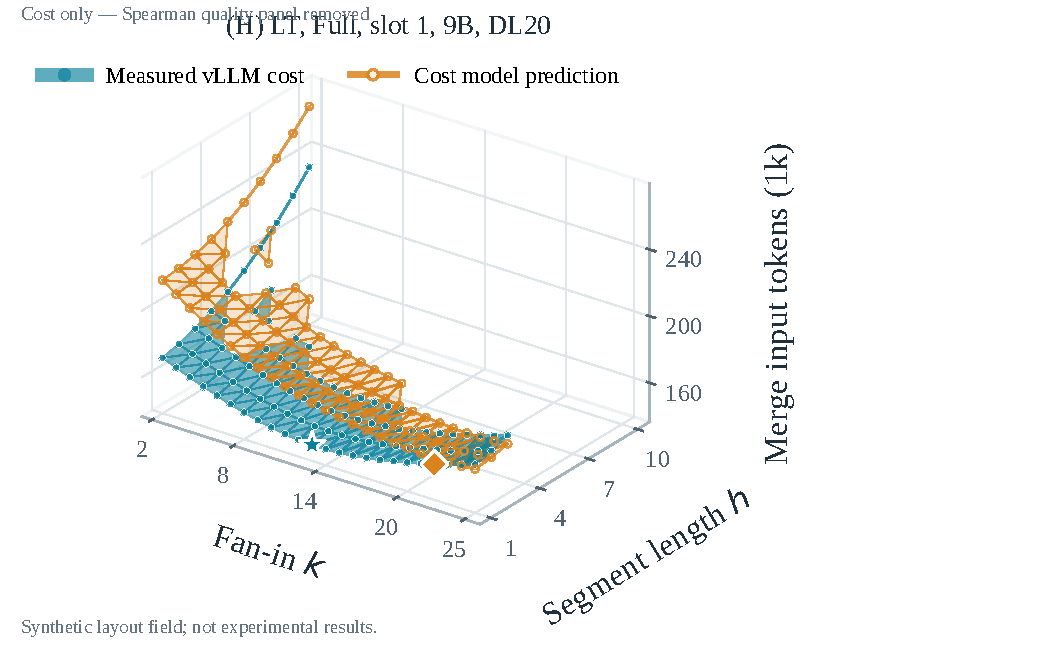
\includegraphics[width=\linewidth]{e2-hero-cost-only.pdf}
  \caption{Single-panel reference style (cost only). Camera \texttt{elev=26}, \texttt{azim=-54}; every $(k,h)$ configuration retains vertex markers like the original \texttt{plot\_surface.py} script.}
  \label{fig:e2-hero}
\end{figure}

\end{document}